% Add to the preamble if not already loaded:
% \usepackage{booktabs}
% \usepackage[table]{xcolor}

% Main text, B2:
\begin{figure}[!t]
  \centering
  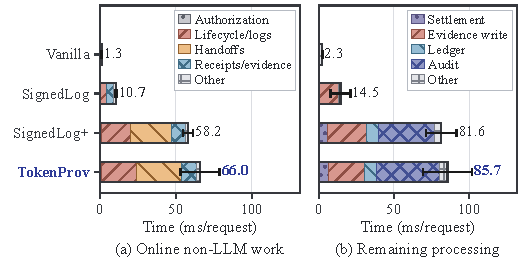
\includegraphics[width=\columnwidth]{b2_reference_cost_breakdown.pdf}
  \caption{Cost breakdown for Qwen3-1.7B at concurrency eight with eight sequential
  calls per request. Stacks show three-round mean component costs; error bars
  show the sample standard deviation of each total across the three round means.}
  \label{fig:b2-cost-breakdown}
\end{figure}

% In the existing appendix, after \appendices:
\section{Additional Cost Breakdown}
\label{app:b2-cost}
Table~\ref{tab:b2-component-breakdown} gives the full breakdown across five models.
Online non-LLM work is $T_{\mathrm{online}}-T_{\mathrm{llm}}$, and remaining
processing is $T_{\mathrm{pipeline}}-T_{\mathrm{online}}$.
The latter includes evidence persistence, audit, settlement, and surrounding
pipeline work, all included in the complete request latency.
% Requires booktabs and xcolor with the table option (or colortbl).
\begin{table*}[!t]
\centering
\caption{TokenProv cost breakdown across models (ms/request; mean $\pm$ sample standard deviation across three rounds).}
\label{tab:b2-component-breakdown}
\footnotesize
\renewcommand{\arraystretch}{1.10}
\begin{tabular*}{\textwidth}{@{\hspace{4pt}}l@{\extracolsep{\fill}}ccccc@{\hspace{4pt}}}
\toprule
\textbf{Component} & \shortstack{\textbf{Qwen3}\\\textbf{1.7B}} & \shortstack{\textbf{Qwen3}\\\textbf{4B}} & \shortstack{\textbf{Phi-3-mini}\\\textbf{3.8B}} & \shortstack{\textbf{DeepSeek-R1-Distill}\\\textbf{Llama-8B}} & \shortstack{\textbf{Qwen3}\\\textbf{14B}} \\
\midrule
\rowcolor{gray!12}
\multicolumn{6}{l}{\textbf{Online non-LLM work}} \\
Authorization & 0.99 $\pm$ 0.14 & 0.84 $\pm$ 0.05 & 0.86 $\pm$ 0.09 & 0.89 $\pm$ 0.07 & 0.88 $\pm$ 0.03 \\
Lifecycle records & 23.00 $\pm$ 4.59 & 18.99 $\pm$ 1.83 & 19.05 $\pm$ 2.44 & 19.12 $\pm$ 2.46 & 19.14 $\pm$ 0.93 \\
$H\!\rightarrow\!B$ handoffs & 15.87 $\pm$ 3.76 & 13.02 $\pm$ 1.58 & 13.10 $\pm$ 2.13 & 12.84 $\pm$ 2.01 & 13.04 $\pm$ 1.24 \\
$B\!\rightarrow\!P$ handoffs & 13.83 $\pm$ 2.64 & 11.63 $\pm$ 1.08 & 11.28 $\pm$ 1.44 & 11.30 $\pm$ 1.57 & 11.42 $\pm$ 0.66 \\
Provider commitments & 1.47 $\pm$ 0.08 & 1.36 $\pm$ 0.13 & 1.41 $\pm$ 0.08 & 1.35 $\pm$ 0.08 & 1.37 $\pm$ 0.06 \\
Receipts & 8.75 $\pm$ 1.63 & 7.10 $\pm$ 0.59 & 6.45 $\pm$ 0.55 & 6.56 $\pm$ 0.90 & 6.82 $\pm$ 0.77 \\
Other online work & 2.07 $\pm$ 0.15 & 1.82 $\pm$ 0.09 & 1.92 $\pm$ 0.09 & 1.91 $\pm$ 0.09 & 1.87 $\pm$ 0.04 \\
\textbf{Online non-LLM total} & 65.98 $\pm$ 12.87 & 54.76 $\pm$ 5.31 & 54.07 $\pm$ 6.73 & 53.98 $\pm$ 7.07 & 54.52 $\pm$ 3.48 \\
\midrule
\rowcolor{gray!12}
\multicolumn{6}{l}{\textbf{Remaining request processing}} \\
Request closure & 1.78 $\pm$ 0.29 & 1.66 $\pm$ 0.06 & 1.53 $\pm$ 0.17 & 1.90 $\pm$ 0.30 & 1.84 $\pm$ 0.17 \\
Merkle construction & 0.70 $\pm$ 0.05 & 0.66 $\pm$ 0.03 & 0.70 $\pm$ 0.02 & 0.67 $\pm$ 0.04 & 0.68 $\pm$ 0.04 \\
Local settlement creation & 3.76 $\pm$ 0.46 & 3.27 $\pm$ 0.11 & 2.98 $\pm$ 0.04 & 3.20 $\pm$ 0.32 & 3.26 $\pm$ 0.29 \\
Evidence persistence & 24.11 $\pm$ 4.93 & 29.06 $\pm$ 8.87 & 23.17 $\pm$ 2.42 & 19.78 $\pm$ 3.87 & 21.16 $\pm$ 1.46 \\
Local ledger & 8.01 $\pm$ 1.22 & 6.88 $\pm$ 0.44 & 7.60 $\pm$ 1.24 & 6.94 $\pm$ 0.94 & 6.89 $\pm$ 0.46 \\
Protocol audit & 41.80 $\pm$ 8.38 & 33.30 $\pm$ 3.87 & 36.05 $\pm$ 3.74 & 34.38 $\pm$ 4.76 & 34.90 $\pm$ 1.82 \\
Other pipeline work & 5.54 $\pm$ 1.21 & 4.32 $\pm$ 0.51 & 4.81 $\pm$ 0.44 & 4.63 $\pm$ 0.52 & 4.81 $\pm$ 0.17 \\
\textbf{Remaining processing total} & 85.70 $\pm$ 16.34 & 79.15 $\pm$ 13.50 & 76.83 $\pm$ 6.99 & 71.49 $\pm$ 10.71 & 73.55 $\pm$ 3.77 \\
\midrule
\textbf{Complete non-LLM total} & 151.68 $\pm$ 29.21 & 133.91 $\pm$ 18.81 & 130.91 $\pm$ 12.00 & 125.47 $\pm$ 17.78 & 128.07 $\pm$ 7.24 \\
\bottomrule
\end{tabular*}
\end{table*}

